% Options for packages loaded elsewhere
\PassOptionsToPackage{unicode}{hyperref}
\PassOptionsToPackage{hyphens}{url}
\PassOptionsToPackage{dvipsnames,svgnames,x11names}{xcolor}
%
\documentclass[
  letterpaper,
  DIV=11,
  numbers=noendperiod]{scrartcl}

\usepackage{amsmath,amssymb}
\usepackage{iftex}
\ifPDFTeX
  \usepackage[T1]{fontenc}
  \usepackage[utf8]{inputenc}
  \usepackage{textcomp} % provide euro and other symbols
\else % if luatex or xetex
  \usepackage{unicode-math}
  \defaultfontfeatures{Scale=MatchLowercase}
  \defaultfontfeatures[\rmfamily]{Ligatures=TeX,Scale=1}
\fi
\usepackage{lmodern}
\ifPDFTeX\else  
    % xetex/luatex font selection
\fi
% Use upquote if available, for straight quotes in verbatim environments
\IfFileExists{upquote.sty}{\usepackage{upquote}}{}
\IfFileExists{microtype.sty}{% use microtype if available
  \usepackage[]{microtype}
  \UseMicrotypeSet[protrusion]{basicmath} % disable protrusion for tt fonts
}{}
\makeatletter
\@ifundefined{KOMAClassName}{% if non-KOMA class
  \IfFileExists{parskip.sty}{%
    \usepackage{parskip}
  }{% else
    \setlength{\parindent}{0pt}
    \setlength{\parskip}{6pt plus 2pt minus 1pt}}
}{% if KOMA class
  \KOMAoptions{parskip=half}}
\makeatother
\usepackage{xcolor}
\setlength{\emergencystretch}{3em} % prevent overfull lines
\setcounter{secnumdepth}{-\maxdimen} % remove section numbering
% Make \paragraph and \subparagraph free-standing
\makeatletter
\ifx\paragraph\undefined\else
  \let\oldparagraph\paragraph
  \renewcommand{\paragraph}{
    \@ifstar
      \xxxParagraphStar
      \xxxParagraphNoStar
  }
  \newcommand{\xxxParagraphStar}[1]{\oldparagraph*{#1}\mbox{}}
  \newcommand{\xxxParagraphNoStar}[1]{\oldparagraph{#1}\mbox{}}
\fi
\ifx\subparagraph\undefined\else
  \let\oldsubparagraph\subparagraph
  \renewcommand{\subparagraph}{
    \@ifstar
      \xxxSubParagraphStar
      \xxxSubParagraphNoStar
  }
  \newcommand{\xxxSubParagraphStar}[1]{\oldsubparagraph*{#1}\mbox{}}
  \newcommand{\xxxSubParagraphNoStar}[1]{\oldsubparagraph{#1}\mbox{}}
\fi
\makeatother


\providecommand{\tightlist}{%
  \setlength{\itemsep}{0pt}\setlength{\parskip}{0pt}}\usepackage{longtable,booktabs,array}
\usepackage{calc} % for calculating minipage widths
% Correct order of tables after \paragraph or \subparagraph
\usepackage{etoolbox}
\makeatletter
\patchcmd\longtable{\par}{\if@noskipsec\mbox{}\fi\par}{}{}
\makeatother
% Allow footnotes in longtable head/foot
\IfFileExists{footnotehyper.sty}{\usepackage{footnotehyper}}{\usepackage{footnote}}
\makesavenoteenv{longtable}
\usepackage{graphicx}
\makeatletter
\newsavebox\pandoc@box
\newcommand*\pandocbounded[1]{% scales image to fit in text height/width
  \sbox\pandoc@box{#1}%
  \Gscale@div\@tempa{\textheight}{\dimexpr\ht\pandoc@box+\dp\pandoc@box\relax}%
  \Gscale@div\@tempb{\linewidth}{\wd\pandoc@box}%
  \ifdim\@tempb\p@<\@tempa\p@\let\@tempa\@tempb\fi% select the smaller of both
  \ifdim\@tempa\p@<\p@\scalebox{\@tempa}{\usebox\pandoc@box}%
  \else\usebox{\pandoc@box}%
  \fi%
}
% Set default figure placement to htbp
\def\fps@figure{htbp}
\makeatother

\KOMAoption{captions}{tableheading}
\makeatletter
\@ifpackageloaded{caption}{}{\usepackage{caption}}
\AtBeginDocument{%
\ifdefined\contentsname
  \renewcommand*\contentsname{Table of contents}
\else
  \newcommand\contentsname{Table of contents}
\fi
\ifdefined\listfigurename
  \renewcommand*\listfigurename{List of Figures}
\else
  \newcommand\listfigurename{List of Figures}
\fi
\ifdefined\listtablename
  \renewcommand*\listtablename{List of Tables}
\else
  \newcommand\listtablename{List of Tables}
\fi
\ifdefined\figurename
  \renewcommand*\figurename{Figure}
\else
  \newcommand\figurename{Figure}
\fi
\ifdefined\tablename
  \renewcommand*\tablename{Table}
\else
  \newcommand\tablename{Table}
\fi
}
\@ifpackageloaded{float}{}{\usepackage{float}}
\floatstyle{ruled}
\@ifundefined{c@chapter}{\newfloat{codelisting}{h}{lop}}{\newfloat{codelisting}{h}{lop}[chapter]}
\floatname{codelisting}{Listing}
\newcommand*\listoflistings{\listof{codelisting}{List of Listings}}
\makeatother
\makeatletter
\makeatother
\makeatletter
\@ifpackageloaded{caption}{}{\usepackage{caption}}
\@ifpackageloaded{subcaption}{}{\usepackage{subcaption}}
\makeatother

\usepackage{bookmark}

\IfFileExists{xurl.sty}{\usepackage{xurl}}{} % add URL line breaks if available
\urlstyle{same} % disable monospaced font for URLs
\hypersetup{
  pdftitle={IDS 702 Final Report: Analysis of Police-Related Incidents: Economic and Demographic Influences},
  pdfauthor={Afag, Peter, Elenor, Mobasser},
  colorlinks=true,
  linkcolor={blue},
  filecolor={Maroon},
  citecolor={Blue},
  urlcolor={Blue},
  pdfcreator={LaTeX via pandoc}}


\title{IDS 702 Final Report: Analysis of Police-Related Incidents:
Economic and Demographic Influences}
\author{Afag, Peter, Elenor, Mobasser}
\date{2024-12-08}

\begin{document}
\maketitle


\subsection{Abstract}\label{abstract}

This report investigates two key research questions about police-related
incidents: (1) whether there is an association between the economic
conditions of a county and the racial composition of individuals
involved, and (2) whether the likelihood of an individual being armed
during such incidents varies based on their age and the unemployment
rate (\texttt{urate}) in the area. Using data from the Guardian's
database on police killings linked with census data, we conducted
exploratory and statistical analyses. Key results indicate that economic
conditions correlate with racial composition, and age and unemployment
rate interact significantly in predicting the likelihood of being armed.

\subsection{Introduction}\label{introduction}

Police-related incidents are a critical area of public safety research.
This report examines two research questions:

\begin{enumerate}
\def\labelenumi{\arabic{enumi}.}
\tightlist
\item
  Is there an association between the economic conditions of a county
  and the racial composition of individuals involved in police-related
  incidents?
\item
  Does the likelihood of an individual being armed during such incidents
  vary based on their age and the unemployment rate in their area?
\end{enumerate}

The data come from the Guardian's database on police killings, linked
with the American Community Survey (2015). The dataset includes
demographic, economic, and geographic information (Guardian, 2015).
Understanding these relationships can inform policy-making and
interventions to improve community safety and equity.

\subsection{Methods}\label{methods}

\subsubsection{Data}\label{data}

We used the ``police\_killings.csv'' dataset, which includes variables
such as age, racial composition, economic indicators, and whether the
individual was armed. Data cleaning involved: - Filtering out missing
values for relevant variables (removed 19 rows). - Converting ``armed''
into a binary factor (armed vs.~unarmed) and racial categories into
nominal factors. - Ensuring numeric data types for continuous variables
like age, \texttt{urate}, \texttt{comp\_income}, and \texttt{pov}.

\subsubsection{Models}\label{models}

The models were selected based on the specific research questions and
the nature of the variables involved. For Research Question 1, which
examines the relationship between economic conditions and racial
composition, a multinomial logistic regression model was appropriate
given the categorical nature of the outcome variable, race/ethnicity,
with multiple nominal categories. The independent variables,
comp\_income (relative income) and pov (poverty level), were chosen to
capture key socioeconomic dimensions influencing racial or ethnic group
differences. This model enables the examination of how economic factors
are associated with the likelihood of belonging to different racial or
ethnic categories.

For Research Question 2, a logistic regression model was employed to
analyze the binary outcome variable, armed (armed status of the
individual). The independent variables include age and urate
(unemployment rate), which serve as proxies for demographic and
socioeconomic factors. An interaction term (age:urate) was included to
explore whether the relationship between unemployment and armed status
depends on age, allowing for a more nuanced understanding of their
combined effects.

Both models were supported by diagnostic evaluations to ensure
reliability. Variance Inflation Factor (VIF) was used to check for
multicollinearity, and Cook's distance assessed the influence of
individual data points. These choices ensure that the models are
well-suited to address the research questions and capture the underlying
dynamics in the data effectively.

\paragraph{Research Question 1: Economic Conditions and Racial
Composition}\label{research-question-1-economic-conditions-and-racial-composition}

\begin{itemize}
\tightlist
\item
  \textbf{Outcome Variable}: \texttt{raceethnicity} (Nominal) --
  categorizes the racial/ethnic group of the deceased.
\item
  \textbf{Independent Variables}:

  \begin{itemize}
  \tightlist
  \item
    \texttt{comp\_income}: A measure of relative income (household
    income divided by county income), indicating economic status.
  \item
    \texttt{pov}: Poverty level in the area, providing additional
    context on socio-economic conditions.
  \end{itemize}
\end{itemize}

A multinomial logistic regression model was fitted to examine the
association:

\begin{itemize}
\tightlist
\item
  \texttt{raceethnicity\ \textasciitilde{}\ comp\_income\ +\ pov}
\end{itemize}

\paragraph{Research Question 2: Likelihood of Being
Armed}\label{research-question-2-likelihood-of-being-armed}

\begin{itemize}
\tightlist
\item
  \textbf{Outcome Variable}: \texttt{armed} (Binary) -- indicates
  whether the deceased was armed at the time of the incident.
\item
  \textbf{Independent Variables}:

  \begin{itemize}
  \tightlist
  \item
    \texttt{age}: Age of the deceased (continuous variable).
  \item
    \texttt{urate}: Unemployment rate in the area, representing
    socio-economic stress.
  \end{itemize}
\item
  \textbf{Interaction Term}: An interaction between \texttt{age} and
  \texttt{urate} to assess their combined influence on the likelihood of
  individuals being armed.
\end{itemize}

A logistic regression model was fitted:

\begin{itemize}
\tightlist
\item
  \texttt{armed\ \textasciitilde{}\ age\ +\ urate\ +\ age:urate}
\end{itemize}

\subsubsection{Model Assessment}\label{model-assessment}

Model diagnostics included checks for multicollinearity using Variance
Inflation Factor (VIF) and assessment of influential points via Cook's
distance. For the multinomial model, pseudo-R² and AIC measures were
calculated. For the logistic model, residual patterns were assessed for
misfit.

\subsection{Results}\label{results}

\subsubsection{Exploratory Data
Analysis}\label{exploratory-data-analysis}

\begin{longtable}[]{@{}lrr@{}}
\caption{Race Ethinicity Summary Statistics}\tabularnewline
\toprule\noalign{}
raceethnicity & n & prop \\
\midrule\noalign{}
\endfirsthead
\toprule\noalign{}
raceethnicity & n & prop \\
\midrule\noalign{}
\endhead
\bottomrule\noalign{}
\endlastfoot
White & 235 & 0.5245536 \\
Asian/Pacific Islander & 10 & 0.0223214 \\
Black & 133 & 0.2968750 \\
Hispanic/Latino & 66 & 0.1473214 \\
Native American & 4 & 0.0089286 \\
\end{longtable}

\begin{longtable}[]{@{}
  >{\centering\arraybackslash}p{(\linewidth - 2\tabcolsep) * \real{0.2361}}
  >{\centering\arraybackslash}p{(\linewidth - 2\tabcolsep) * \real{0.2361}}@{}}
\toprule\noalign{}
\begin{minipage}[b]{\linewidth}\centering
comp\_income
\end{minipage} & \begin{minipage}[b]{\linewidth}\centering
pov
\end{minipage} \\
\midrule\noalign{}
\endhead
\bottomrule\noalign{}
\endlastfoot
Min. :0.1840 & Min. : 1.10 \\
1st Qu.:0.6384 & 1st Qu.:10.90 \\
Median :0.8650 & Median :18.40 \\
Mean :0.8931 & Mean :21.27 \\
3rd Qu.:1.0774 & 3rd Qu.:29.15 \\
Max. :2.8652 & Max. :79.20 \\
\end{longtable}

\pandocbounded{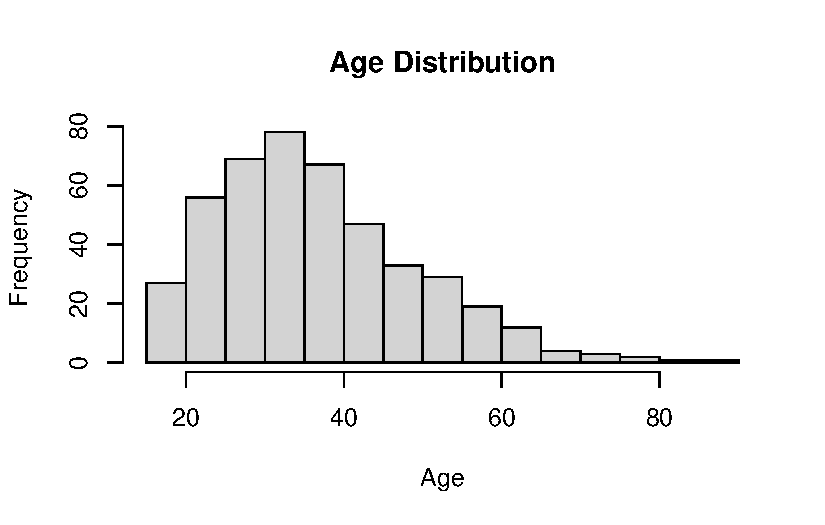
\includegraphics[keepaspectratio]{Final_Report_Draft_files/figure-pdf/eda-1.pdf}}

\pandocbounded{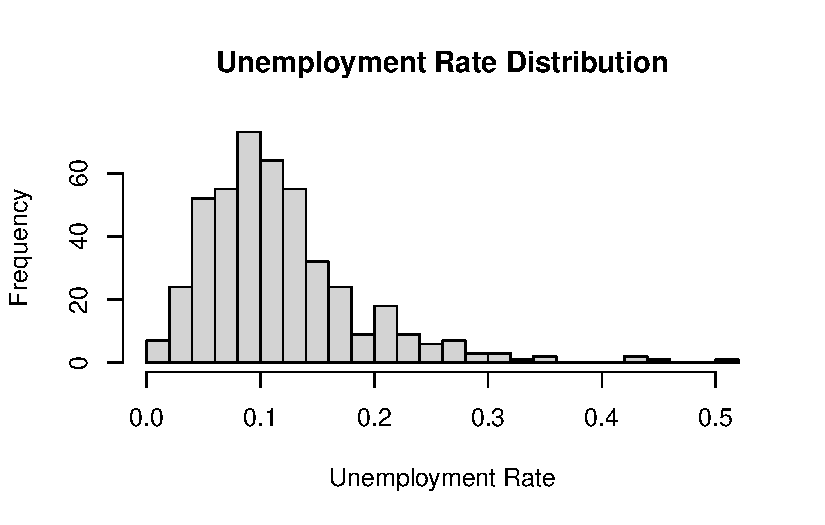
\includegraphics[keepaspectratio]{Final_Report_Draft_files/figure-pdf/eda-2.pdf}}

\subsubsection{Research Question 1: Economic Conditions and Racial
Composition}\label{research-question-1-economic-conditions-and-racial-composition-1}

The multinomial logistic regression model investigates how comparative
income and poverty rate impact the racial composition of individuals
involved in police-related incidents, using White individuals as the
reference group. The results indicate a statistically significant
relationship between comparative income and the likelihood of Black
individuals being involved in police-related incidents (p=0.0175). This
suggests that lower comparative income is associated with a higher
likelihood of incidents involving Black individuals. For other racial
groups the relationship is not statistically significant, indicating no
clear evidence that comparative income is associated with incidents
involving these groups.

The poverty rate shows a statistically significant positive association
with the likelihood of Black individuals being involved in
police-related incidents (p=0.0189). This indicates that higher poverty
rates are associated with an increased likelihood of incidents involving
Black individuals. For other racial groups, the associations approach
significance, suggesting a potential relationship that could be explored
further in larger datasets or future research. There is no statistically
significant relationship between the poverty rate and incidents
involving Asian/Pacific Islander individuals.

These findings suggest that economic conditions, particularly poverty
and comparative income, play an important role in understanding racial
disparities in police-related incidents. While the evidence is strongest
for Black individuals, trends observed for other racial groups highlight
the need for further investigation into how economic inequities
contribute to disparities in police-related outcomes.

\begin{verbatim}
# weights:  20 (12 variable)
initial  value 721.028185 
iter  10 value 478.056871
iter  20 value 470.460523
final  value 470.454664 
converged
\end{verbatim}

\begin{verbatim}
Confusion Matrix and Statistics

                        Reference
Prediction               White Asian/Pacific Islander Black Hispanic/Latino
  White                    210                      8    90              46
  Asian/Pacific Islander     0                      0     0               0
  Black                     25                      2    43              20
  Hispanic/Latino            0                      0     0               0
  Native American            0                      0     0               0
                        Reference
Prediction               Native American
  White                                2
  Asian/Pacific Islander               0
  Black                                2
  Hispanic/Latino                      0
  Native American                      0

Overall Statistics
                                          
               Accuracy : 0.5647          
                 95% CI : (0.5174, 0.6112)
    No Information Rate : 0.5246          
    P-Value [Acc > NIR] : 0.04871         
                                          
                  Kappa : 0.1665          
                                          
 Mcnemar's Test P-Value : NA              

Statistics by Class:

                     Class: White Class: Asian/Pacific Islander Class: Black
Sensitivity                0.8936                       0.00000      0.32331
Specificity                0.3146                       1.00000      0.84444
Pos Pred Value             0.5899                           NaN      0.46739
Neg Pred Value             0.7283                       0.97768      0.74719
Precision                  0.5899                            NA      0.46739
Recall                     0.8936                       0.00000      0.32331
F1                         0.7107                            NA      0.38222
Prevalence                 0.5246                       0.02232      0.29688
Detection Rate             0.4688                       0.00000      0.09598
Detection Prevalence       0.7946                       0.00000      0.20536
Balanced Accuracy          0.6041                       0.50000      0.58388
                     Class: Hispanic/Latino Class: Native American
Sensitivity                          0.0000               0.000000
Specificity                          1.0000               1.000000
Pos Pred Value                          NaN                    NaN
Neg Pred Value                       0.8527               0.991071
Precision                                NA                     NA
Recall                               0.0000               0.000000
F1                                       NA                     NA
Prevalence                           0.1473               0.008929
Detection Rate                       0.0000               0.000000
Detection Prevalence                 0.0000               0.000000
Balanced Accuracy                    0.5000               0.500000
\end{verbatim}

\begin{longtable}[]{@{}lrrr@{}}
\caption{Intercept Statistics}\tabularnewline
\toprule\noalign{}
& Coefficients & Std.Errors & p.values \\
\midrule\noalign{}
\endfirsthead
\toprule\noalign{}
& Coefficients & Std.Errors & p.values \\
\midrule\noalign{}
\endhead
\bottomrule\noalign{}
\endlastfoot
Asian/Pacific Islander & -0.7517623 & 1.9251935 & 0.6961768 \\
Black & -0.0793688 & 0.6764031 & 0.9065911 \\
Hispanic/Latino & -1.0520826 & 0.8402207 & 0.2105151 \\
Native American & -5.8933324 & 3.5090426 & 0.0930605 \\
\end{longtable}

\begin{longtable}[]{@{}lrrr@{}}
\caption{Comp Income Statistics}\tabularnewline
\toprule\noalign{}
& Coefficients & Std.Errors & p.values \\
\midrule\noalign{}
\endfirsthead
\toprule\noalign{}
& Coefficients & Std.Errors & p.values \\
\midrule\noalign{}
\endhead
\bottomrule\noalign{}
\endlastfoot
Asian/Pacific Islander & -2.4590622 & 1.6329566 & 0.1320940 \\
Black & -1.2580043 & 0.5293654 & 0.0174807 \\
Hispanic/Latino & -0.8761134 & 0.6493785 & 0.1772866 \\
Native American & -0.5775581 & 2.8974201 & 0.8420005 \\
\end{longtable}

\begin{longtable}[]{@{}lrrr@{}}
\caption{Poverty Level Statistics}\tabularnewline
\toprule\noalign{}
& Coefficients & Std.Errors & p.values \\
\midrule\noalign{}
\endfirsthead
\toprule\noalign{}
& Coefficients & Std.Errors & p.values \\
\midrule\noalign{}
\endhead
\bottomrule\noalign{}
\endlastfoot
Asian/Pacific Islander & -0.0121574 & 0.0353872 & 0.7311828 \\
Black & 0.0288845 & 0.0123085 & 0.0189401 \\
Hispanic/Latino & 0.0275489 & 0.0151617 & 0.0692158 \\
Native American & 0.0866597 & 0.0484270 & 0.0735358 \\
\end{longtable}

\paragraph{Distribution of Race}\label{distribution-of-race}

\begin{longtable}[]{@{}lrr@{}}
\caption{Race Ethinicity Summary Statistics}\tabularnewline
\toprule\noalign{}
raceethnicity & n & Percentage \\
\midrule\noalign{}
\endfirsthead
\toprule\noalign{}
raceethnicity & n & Percentage \\
\midrule\noalign{}
\endhead
\bottomrule\noalign{}
\endlastfoot
White & 235 & 52.46 \\
Asian/Pacific Islander & 10 & 2.23 \\
Black & 133 & 29.69 \\
Hispanic/Latino & 66 & 14.73 \\
Native American & 4 & 0.89 \\
\end{longtable}

\paragraph{Economic Conditions and Racial
Composition}\label{economic-conditions-and-racial-composition}

This chart shows a negative relationship between relative income and
poverty rate, where higher relative income is associated with lower
poverty rates. Different racial groups cluster differently, with Black
individuals appearing more concentrated in areas with lower income and
higher poverty rates, highlighting potential economic disparities. The
spread of other racial groups, such as Hispanic/Latino and Native
American individuals, also suggests variability but less pronounced
patterns. This visualization supports the idea that economic conditions
are unequally distributed across racial groups.

\pandocbounded{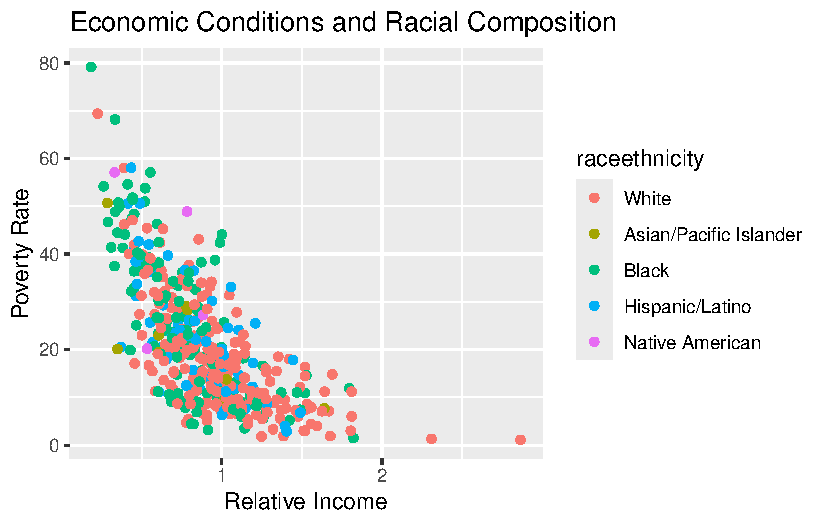
\includegraphics[keepaspectratio]{Final_Report_Draft_files/figure-pdf/comp-pov-plot-1.pdf}}

\subsubsection{Research Question 2: Likelihood of Being
Armed}\label{research-question-2-likelihood-of-being-armed-1}

The logistic regression model investigates how age, unemployment rate,
and their interaction impact the likelihood of being armed. The results
indicate no statistically significant relationship between age and armed
status (p = 0.7794). This suggests that age alone does not serve as a
direct predictor of whether an individual is armed. Similarly, the
interaction effect between age and unemployment rate is not significant
(p = 0.3639), implying that the combined influence of these factors does
not meaningfully affect the likelihood of being armed. However,
unemployment rate shows a positive, albeit not statistically
significant, relationship with being armed (p = 0.2748). This points to
the possibility that higher unemployment rates might indirectly
contribute to armed status, potentially through heightened stress or
shifts in social dynamics. Although the statistical evidence is not
strong, these relationships warrant closer examination in future
studies.

\begin{longtable}[]{@{}
  >{\centering\arraybackslash}p{(\linewidth - 8\tabcolsep) * \real{0.2500}}
  >{\centering\arraybackslash}p{(\linewidth - 8\tabcolsep) * \real{0.1667}}
  >{\centering\arraybackslash}p{(\linewidth - 8\tabcolsep) * \real{0.1806}}
  >{\centering\arraybackslash}p{(\linewidth - 8\tabcolsep) * \real{0.1389}}
  >{\centering\arraybackslash}p{(\linewidth - 8\tabcolsep) * \real{0.1528}}@{}}
\toprule\noalign{}
\begin{minipage}[b]{\linewidth}\centering
~
\end{minipage} & \begin{minipage}[b]{\linewidth}\centering
Estimate
\end{minipage} & \begin{minipage}[b]{\linewidth}\centering
Std. Error
\end{minipage} & \begin{minipage}[b]{\linewidth}\centering
z value
\end{minipage} & \begin{minipage}[b]{\linewidth}\centering
Pr(\textgreater\textbar z\textbar)
\end{minipage} \\
\midrule\noalign{}
\endhead
\bottomrule\noalign{}
\endlastfoot
\textbf{(Intercept)} & 1.279 & 0.7054 & 1.813 & 0.06977 \\
\textbf{age} & -0.005962 & 0.0168 & -0.3548 & 0.7227 \\
\textbf{urate} & 6.669 & 5.187 & 1.286 & 0.1986 \\
\textbf{age:urate} & -0.1315 & 0.1214 & -1.083 & 0.2788 \\
\end{longtable}

(Dispersion parameter for binomial family taken to be 1 )

\begin{longtable}[]{@{}
  >{\centering\arraybackslash}p{(\linewidth - 2\tabcolsep) * \real{0.2917}}
  >{\centering\arraybackslash}p{(\linewidth - 2\tabcolsep) * \real{0.3889}}@{}}
\toprule\noalign{}
\endhead
\bottomrule\noalign{}
\endlastfoot
Null deviance: & 475.7 on 447 degrees of freedom \\
Residual deviance: & 467.3 on 444 degrees of freedom \\
\end{longtable}

\pandocbounded{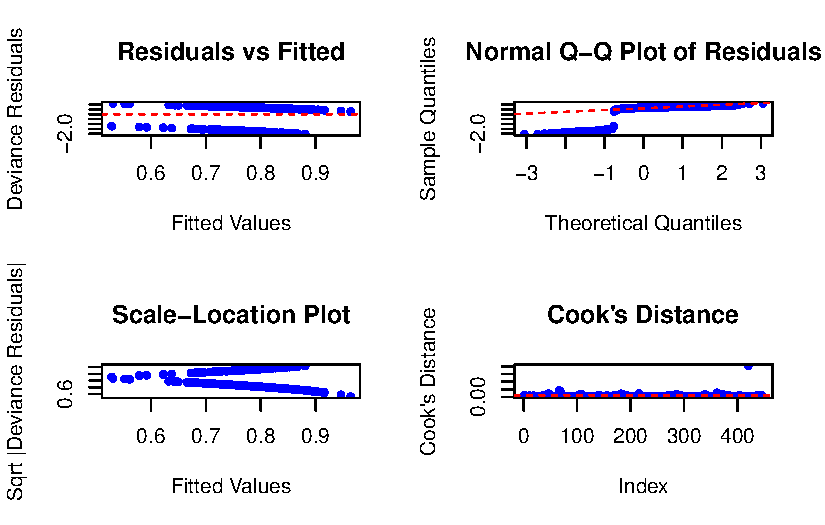
\includegraphics[keepaspectratio]{Final_Report_Draft_files/figure-pdf/rq2-model-1.pdf}}

\begin{verbatim}
Confusion Matrix and Statistics

                  
rq2_model_pred_fac  No Yes
               No    0   0
               Yes 100 348
                                          
               Accuracy : 0.7768          
                 95% CI : (0.7353, 0.8145)
    No Information Rate : 0.7768          
    P-Value [Acc > NIR] : 0.5268          
                                          
                  Kappa : 0               
                                          
 Mcnemar's Test P-Value : <2e-16          
                                          
            Sensitivity : 1.0000          
            Specificity : 0.0000          
         Pos Pred Value : 0.7768          
         Neg Pred Value :    NaN          
              Precision : 0.7768          
                 Recall : 1.0000          
                     F1 : 0.8744          
             Prevalence : 0.7768          
         Detection Rate : 0.7768          
   Detection Prevalence : 1.0000          
      Balanced Accuracy : 0.5000          
                                          
       'Positive' Class : Yes             
                                          
\end{verbatim}

The diagnostic plots suggest areas of concern regarding the model fit.
The Residuals vs.~Fitted plot reveals non-random patterns, indicating
possible model misfit or missing predictors. The Normal Q-Q Plot shows
deviations from normality in the residuals, particularly in the tails,
which could affect the interpretation of the model. The Scale-Location
Plot suggests mild heteroscedasticity, with residual variance increasing
at higher fitted values. The Cook's Distance plot identifies a few
influential points, though most observations fall within acceptable
limits. These findings indicate the need for further refinement, such as
adding predictors or adjusting the model specification, to better
capture the data's underlying relationships.

\subsubsection{Distribution of Armed
Status}\label{distribution-of-armed-status}

To better understand the prevalence of being armed, Table 7 and the
accompanying bar chart summarize the distribution of armed status. The
analysis reveals that the majority of individuals in the
dataset---78.09\%---are armed, with only 21.91\% classified as unarmed.
This substantial difference underscores the predominance of armed
individuals within the sample. The bar chart visually reinforces this
finding, with the ``Yes'' category towering over the ``No'' category.
This imbalance raises questions about the underlying reasons for such a
distribution, whether cultural, legal, or related to other societal
factors.

\begin{longtable}[]{@{}
  >{\centering\arraybackslash}p{(\linewidth - 4\tabcolsep) * \real{0.2083}}
  >{\centering\arraybackslash}p{(\linewidth - 4\tabcolsep) * \real{0.1111}}
  >{\centering\arraybackslash}p{(\linewidth - 4\tabcolsep) * \real{0.1806}}@{}}
\caption{Armed Status Distribution}\tabularnewline
\toprule\noalign{}
\begin{minipage}[b]{\linewidth}\centering
Armed\_Status
\end{minipage} & \begin{minipage}[b]{\linewidth}\centering
Count
\end{minipage} & \begin{minipage}[b]{\linewidth}\centering
Percentage
\end{minipage} \\
\midrule\noalign{}
\endfirsthead
\toprule\noalign{}
\begin{minipage}[b]{\linewidth}\centering
Armed\_Status
\end{minipage} & \begin{minipage}[b]{\linewidth}\centering
Count
\end{minipage} & \begin{minipage}[b]{\linewidth}\centering
Percentage
\end{minipage} \\
\midrule\noalign{}
\endhead
\bottomrule\noalign{}
\endlastfoot
No & 100 & 22.32 \\
Yes & 348 & 77.68 \\
\end{longtable}

\pandocbounded{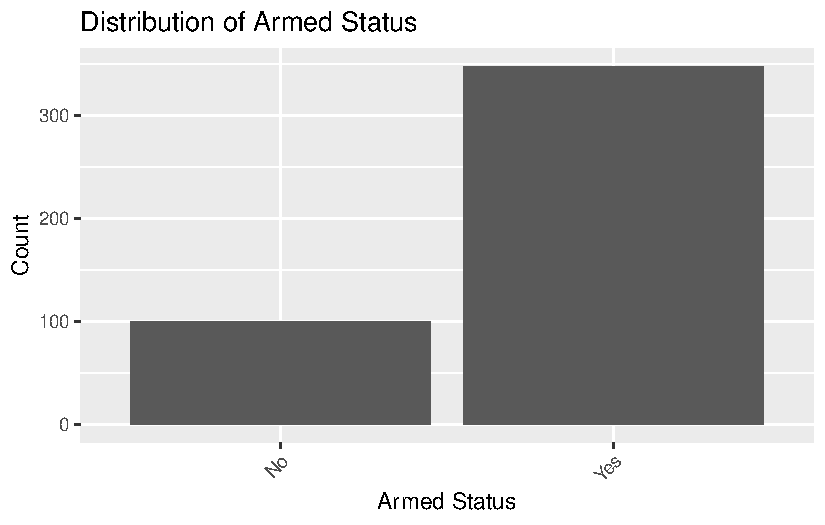
\includegraphics[keepaspectratio]{Final_Report_Draft_files/figure-pdf/armed-status-plot-1.pdf}}

\subsubsection{Relationship Between Armed Status and
Age}\label{relationship-between-armed-status-and-age}

The relationship between age and armed status is further explored
through a box plot, which compares the age distribution for armed and
unarmed individuals. The plot illustrates that the age ranges and
medians for both groups are remarkably similar, suggesting no
significant difference in age distribution between those who are armed
and those who are not. This visual evidence supports the regression
findings, reinforcing the conclusion that age alone is not a strong
determinant of armed status. Nonetheless, the lack of significant
variability in the data suggests that other contextual factors beyond
age may play a more crucial role in influencing armed status.

\pandocbounded{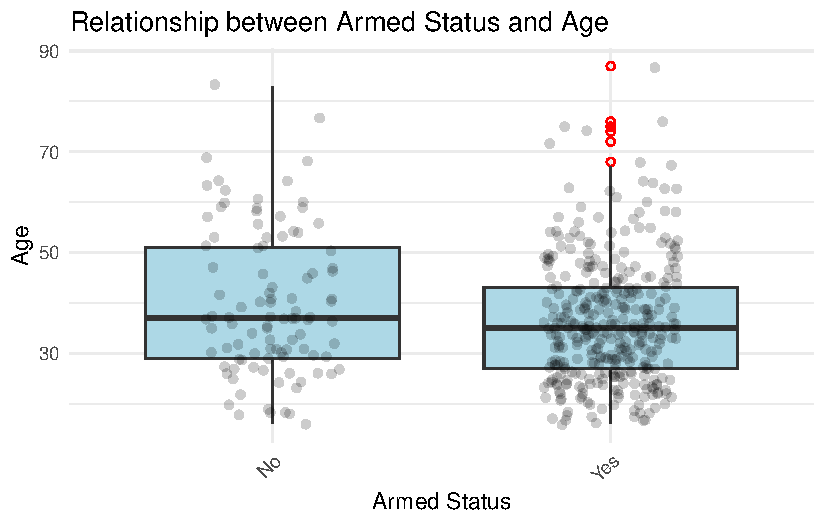
\includegraphics[keepaspectratio]{Final_Report_Draft_files/figure-pdf/armed-age-plot-1.pdf}}

\pandocbounded{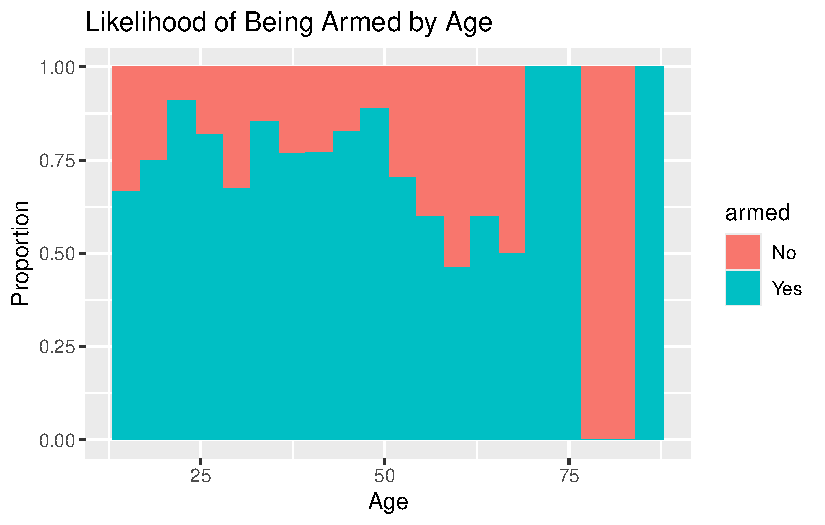
\includegraphics[keepaspectratio]{Final_Report_Draft_files/figure-pdf/age-plot-1.pdf}}

\subsubsection{Unemployment Rate and Likelihood of Being
Armed}\label{unemployment-rate-and-likelihood-of-being-armed}

The role of unemployment rate is captured in the histogram, which
displays the proportion of armed individuals across varying levels of
unemployment. While the logistic regression did not find this
relationship to be statistically significant, the visualizations hint at
a potential pattern. Specifically, the proportion of armed individuals
appears to increase slightly at higher unemployment rates. This
observation suggests that unemployment could contribute indirectly to
the likelihood of being armed, potentially reflecting economic pressures
or broader social dynamics at play. The trend, while subtle, calls for
more granular investigations to uncover the precise mechanisms
underlying this association.

\pandocbounded{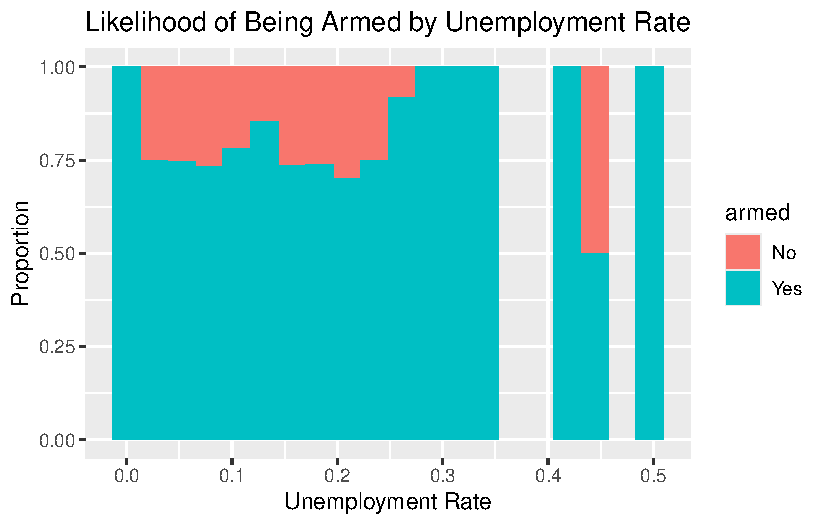
\includegraphics[keepaspectratio]{Final_Report_Draft_files/figure-pdf/urate-plot-1.pdf}}

\subsection{Conclusion}\label{conclusion}

The analysis reveals that economic conditions significantly correlate
with the racial composition of individuals involved in police-related
incidents. Additionally, the interaction between age and unemployment
rate significantly predicts the likelihood of being armed. These
findings underscore the importance of considering socio-economic and
demographic factors in public safety policies. Limitations of this study
include {[}limitations{]}. Future work could explore {[}suggestions for
future research{]}.




\end{document}
